\pdfminorversion=4
\documentclass[xcolor=dvipsnames]{beamer} 
%\usetheme{Warsaw} 
\usecolortheme[RGB={0,99,0}]{structure}
\usetheme{Darmstadt} 
\usepackage[utf8]{inputenc}
\usepackage[spanish]{babel}
%\providecommand{\abs}[1]{\lvert#1\rvert}
%\renewcommand{\frametitle}{\frametitle{\subsecname}} 
%\setbeamercovered{transparent} 
\usepackage{tikz}
%\usepackage{enumitem}
%\setenumerate[1]{label=\arabic*.}
\newcounter{ResumeEnumerate}
\begin{document}
\title{Introducción a Python Científico}
\logo{  \includegraphics[width=1cm,height=1cm,keepaspectratio]{Imagenes/logo.jpg}}
\subtitle{Presentación - Puerto Madryn, del 10 al 14 de marzo}
\date{\scalebox{3}{\insertlogo}}

%---------------------------------------------------------------------------
\begin{frame}
\titlepage
\end{frame}

%---------------------------------------------------------------------------
\section{Qu\'e es Python?}

\begin{frame}{¿Qu\'e es Python ?}
	Python es un lenguaje de programación dinámico de propósito general. Algunas de sus características son:
	\begin{itemize}
		\item Fácil de aprender.
		\item Es todo terreno. 
		\item Es libre, con un ecosistema libre.
		\item Interactivo, pueden verse resultados rápidamente.
		\item Puede comunicarse con otros lenguajes fácilmente.(R, Fortran, C, C++, LaTeX)
		\item Argentina tiene la comunidad hispanohablante más grande.
		\item Muy bien documentado.
	\end{itemize}
% \begin{figure}[h]
%	\begin{center}
%		\includegraphics[scale = 0.4]{venn.png}
%	\end{center}
	%\caption{Landmarks de tipo II, imagen obtenida de ~\cite{Gonzalez2011} }
%\end{figure}
%Hacer diagrama de venn
\end{frame}

%---------------------------------------------------------------------------
\begin{frame}{Qu\'e podemos hacer con Python?}
 \begin{figure}[h]
%	\begin{center}
		\includegraphics[scale = 0.25]{Imagenes/quehacer5.png}
%	\end{center}
	%\caption{Landmarks de tipo II, imagen obtenida de ~\cite{Gonzalez2011} }
\end{figure}
\end{frame}

\begin{frame}{Qu\'e podemos hacer con Python? (Cont.)}

 \begin{figure}[h]
%	\begin{center}
		\includegraphics[scale = 0.2]{Imagenes/quehacer2.png}
%	\end{center}
	%\caption{Landmarks de tipo II, imagen obtenida de ~\cite{Gonzalez2011} }
\end{figure}
\end{frame}



%---------------------------------------------------------------------------
\begin{frame}{Qu\'e podemos hacer con Python? (Cont.)}

 \begin{figure}[h]
%	\begin{center}
		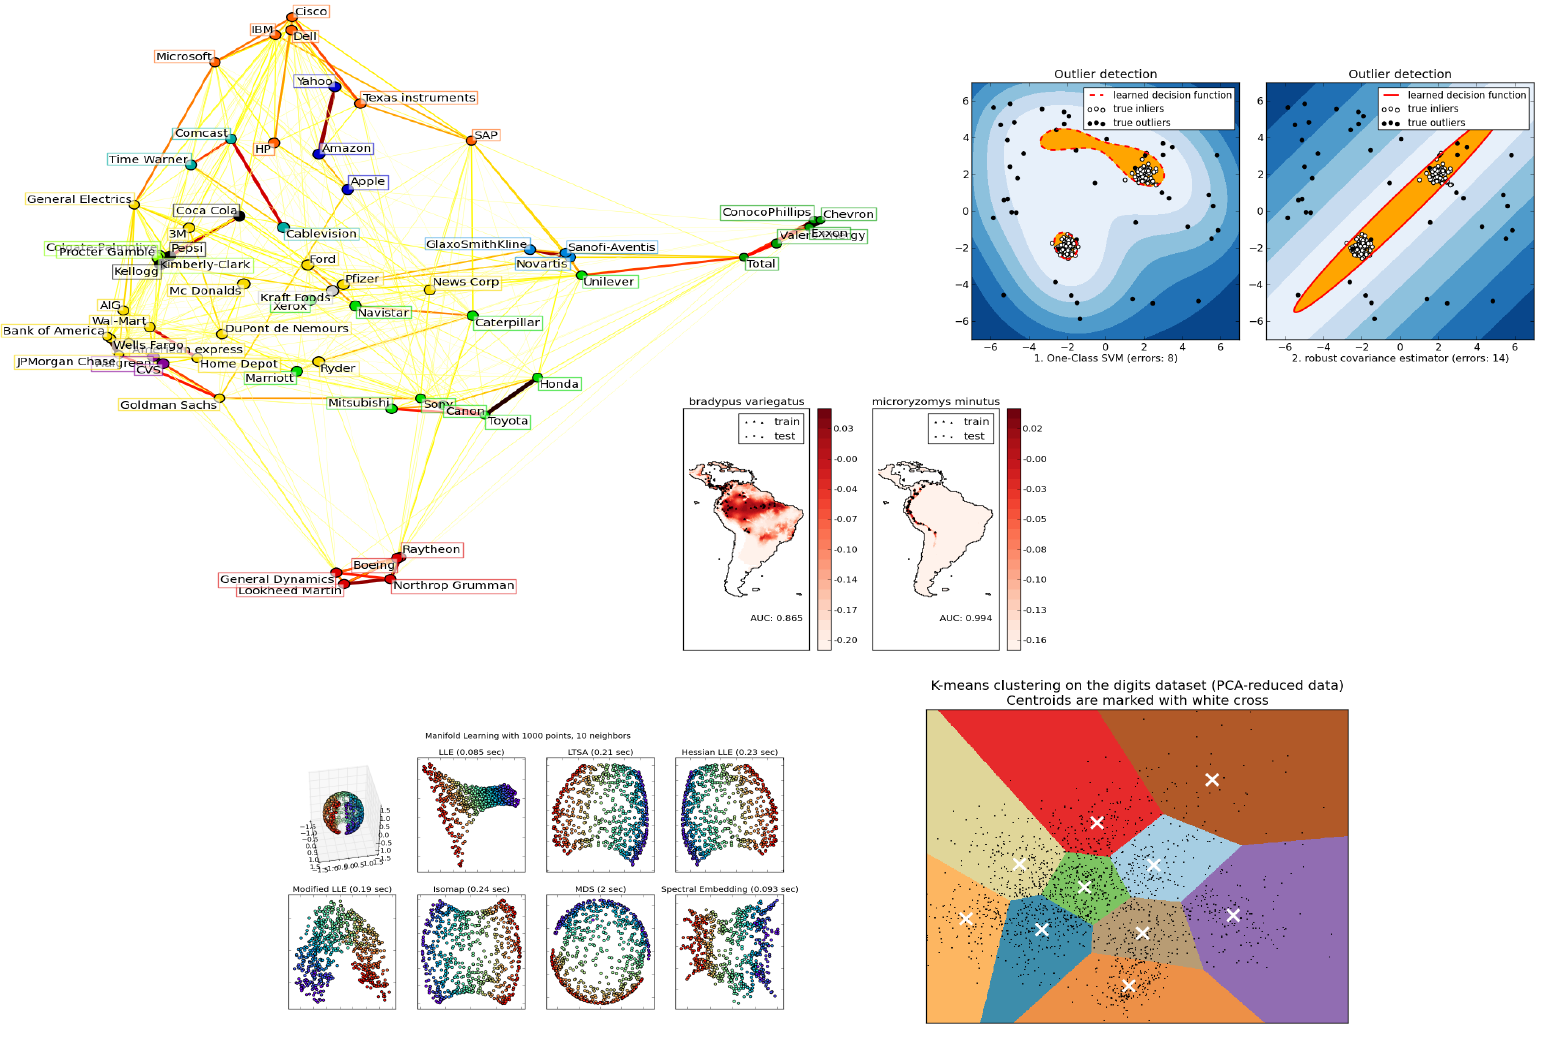
\includegraphics[scale = 0.18]{Imagenes/quehacer3.png}
%	\end{center}
	%\caption{Landmarks de tipo II, imagen obtenida de ~\cite{Gonzalez2011} }
\end{figure}
\end{frame}


%---------------------------------------------------------------------------
\begin{frame}{Qu\'e podemos hacer con Python? (Cont.)}

 \begin{figure}[h]
%	\begin{center}
		\includegraphics[scale = 0.22]{Imagenes/quehacer4.png}
%	\end{center}
	%\caption{Landmarks de tipo II, imagen obtenida de ~\cite{Gonzalez2011} }
\end{figure}
\end{frame}


%---------------------------------------------------------------------------
\section{Cómo esta compuesto Python Científico?}
\begin{frame}{Núcleo de Python Científico}
	\begin{itemize}
	\item \emph{NumPy} (\url{http://www.numpy.org/})
	\item \emph{SciPy} (\url{http://scipy.org/scipylib/index.html})
	\item \emph{Matplotlib} (\url{http://matplotlib.org/})
	\item \emph{IPython} (\url{http://ipython.org/})
\end{itemize}
\end{frame}

%---------------------------------------------------------------------------
\begin{frame}{Otras bibliotecas interesantes}
	\begin{itemize}
		\item \emph{pandas} (\url{http://pandas.pydata.org/})
		\item \emph{MayaVi} (\url{http://docs.enthought.com/mayavi/mayavi/})
		\item \emph{scikit-learn} (\url{http://scikit-learn.org/stable/index.html})
		\item \emph{scikit-image} (\url{http://scikit-image.org/})
		\item \emph{BioPython} (\url{http://biopython.org/wiki/Main_Page})
	\end{itemize}
\end{frame}

\section{Instalación}
%---------------------------------------------------------------------------
\begin{frame}[fragile]{Cómo se instala todo esto?!}
	\begin{itemize}
		\item Linux
		\begin{itemize}
			\item \begin{verbatim} # apt-get install ... \end{verbatim}
			\item \begin{verbatim} # pacman -S ... \end{verbatim}
			\item \begin{verbatim} # pip install ...\end{verbatim}
		\end{itemize}
		\item Multiplataforma
		\begin{itemize}
			\item Anaconda
			\item Canopy
			\item Python(x,y)
		\end{itemize}
		\item Mac OS
		\begin{itemize}
			\item SciPy SuperPack
		\end{itemize}
	\end{itemize}
\end{frame}
%---------------------------------------------------------------------------
\begin{frame}[fragile]{Instalando Anaconda ...}
	 \begin{figure}[h]
%	\begin{center}
		\includegraphics[scale = 0.22]{Imagenes/instalacion.png}
%	\end{center}
	%\caption{Landmarks de tipo II, imagen obtenida de ~\cite{Gonzalez2011} }
\end{figure}
\end{frame}
%---------------------------------------------------------------------------
\begin{frame}{Instalando Anaconda ... (Cont.)}
Qué es lo que acabamos de instalar?
\begin{itemize}
	\item Spyder.
	\item Ipython Notebook.
	\item Ipython QTConsole.
	\item Ipython.
	\item Anaconda Console.
	\item Wakari.
\end{itemize}
\end{frame}
%---------------------------------------------------------------------------
\section{A programar ...}
\begin{frame}{A programar ...}
 \begin{figure}[h]
%	\begin{center}
		\includegraphics[scale = 0.25]{Imagenes/xkcd.png}
%	\end{center}
	%\caption{Landmarks de tipo II, imagen obtenida de ~\cite{Gonzalez2011} }
\end{figure}
\end{frame}

\end{document}

